
Stemming from our case-study, this section presents the SEEDS method in a generalised form. 

SEEDS entails using four practical tools: (a) a questionnaire; (b) a checklist; (c) a decision-tree; (d) an analysis framework. The remainder of this section introduces the SEEDS method in phases. Sections \ref{quest} to \ref{fw} provide additional details on the questionnaire, checklist, decision-tree and evaluation framework.
%

 \begin{figure}[h!]
%\hspace{-.6cm}
%\begin{sideways}
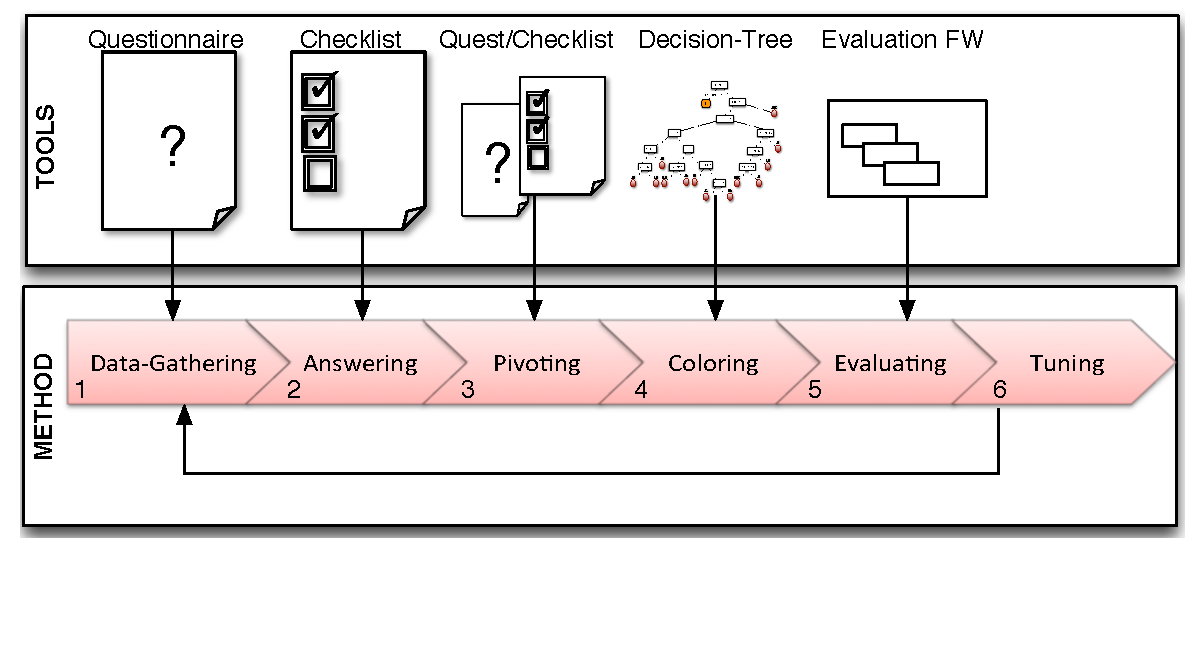
\includegraphics[width=5.3in]{odessamethod}%
%\end{sideways}
\caption{The SEEDS Method: Tools and Phases.}\label{SEEDS}
\end{figure}
%First, a checklist is used to gather the essential organisational data to characterise an observable community.  The questionnaire can also be fed to members of the observed community to gather the needed data.
%\subsection{Method Phases}
%ELABORATE\\
SEEDS unfolds in the following phases:

\begin{enumerate}

\item \emph{\bf Data-Gathering:} \emph{Use questionnaire to gather needed community data.}
Missing data can be gathered by directly surveying (e.g.~with online forms) members of the community under observation. Alternatively, quantitative mechanisms can be used, such as Social-Network Analysis (SNA) \cite{Rosso2009}. Table \ref{quest} presents the SEEDS questionnaire. Each question is the result of analysis and brainstorming sessions with industrial partners and other cooperators. The questionnaire refinement exercise was aimed at pinpointing the right questions for SEEDS.

\item \emph{\bf Answering:} \emph{Use checklist to get attributes value.}
The checklist must then be filled out using the data gathered through our questionnaire. The checklist is a lightweight mechanism to analysing observable development communities, rather than using complex coding schemes on available evidence, as seen previously in literature \cite{Rosso2009,Hustad2010}. Fig.~\ref{checklist} shows the list. Each item within the checklist is a key defining attribute for a community type (see Table \ref{commtypes}), according to data in \cite{ossslr}. Available data must enable answering all the questions in the questionnaire.

\item \emph{\bf Pivoting:} \emph{Double-check questionnaire and checklist to identify multiple answers.}
Pivot-points are points in the checklist that can have multiple answers. A community is a fluid, dynamically evolving emergent property of cooperating organisations. We found in practice multiple community archetypes emerging at the same time where managers assumed there were none. Pivot-points indicate either: (a) there is a conflict or inconsistency in the analysed community \emph{snapshot}; or (b) another community (or sub-community) exists within the observed community, strong enough to cause conflicts and inconsistencies. For example an observed community might show both ``dispersed'' sites and ``non-dispersed'' sites. This means that the community is the sum of multiple communities, based on the remaining attributes.

\item \emph{\bf Coloring:} \emph{Use checklist to ``color'' the SEEDS decision-tree.}
Answers from the checklist allow immediate mapping to the decision-tree to uncover community types and additional attributes present in the observed community. A community \emph{snapshot} has been obtained.

\item \emph{\bf Evaluating:} \emph{Use evaluation framework to analyse the \emph{snapshot} found.}
The framework shown in Fig.~\ref{fwpic} provides a lens to interpret the \emph{\emph{snapshots}} from multiple angles. In particular, the framework allows to pinpoint hazardous organisational barriers and assist in organisational decision-making by means of the \emph{snapshot}. For example, the evaluation framework allowed us to discover a hazardous communication barrier and the means to mitigate it.

\item \emph{\bf Tuning:} \emph{Use evaluation and literature \cite{ossslr} to act on the community.}
\emph{\emph{Snapshots}} can be evaluated to steer community operations. SEEDS allows to pinpoint critical information with which to act on the community, by ``tuning'' desired properties. For example, in practice we found an organisational barrier that can be mitigated by adding a knowledge community within the analysed \emph{snapshot}.

\end{enumerate}
\begin{table}
\hspace{1cm}
%\begin{sideways}
%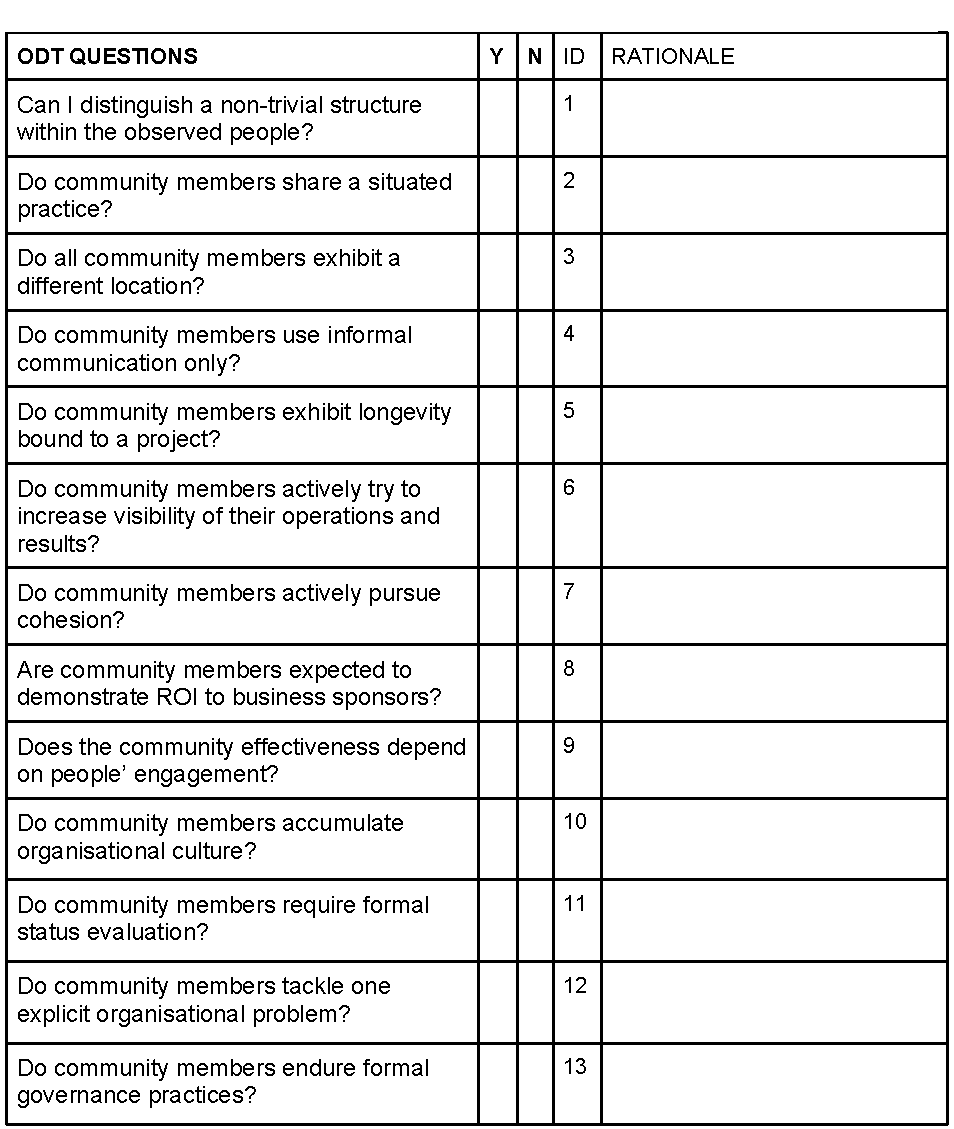
\includegraphics[width=5.44in]{quest}%
%\end{sideways}

\begin{tabular}{|>{\raggedright}p{11cm}|>{\raggedright}p{1.5cm}|}
\hline 
\textbf{Question} & \textbf{Answer}\tabularnewline
\hline 
\emph{Can you distinguish an organised structure across yourself and
your colleagues?} & \tabularnewline
\hline 
\emph{Do you and the colleagues you work with work in the same single
site?} & \tabularnewline
\hline 
\emph{Do you work in a highly-distributed setting with few teams or
colleagues per location?} & \tabularnewline
\hline 
\emph{Do you and your fellow colleagues interact informally only?} & \tabularnewline
\hline 
\emph{Do you work on time-bound projects?} & \tabularnewline
\hline 
\emph{Do you and your colleagues disseminate or increase the visibility
of your work? } & \tabularnewline
\hline 
\emph{Do you and your colleagues actively try to team-build? } & \tabularnewline
\hline 
\emph{Do you need to explicitly demonstrate ROI to your organization? } & \tabularnewline
\hline 
\emph{Does the success of your community depend on your engagement? } & \tabularnewline
\hline 
\emph{Do you and your colleagues actively gather and share organisational
culture (e.g.~best-practices, common problems)?} & \tabularnewline
\hline 
\emph{Were you and your colleagues formally evaluated and qualified
when enrolled in the organisation? } & \tabularnewline
\hline 
\emph{Do you and your colleagues work against the same specific organisational
problem? } & \tabularnewline
\hline 
\emph{Do you and your colleagues undergo rigid governance models imposed
by your organisation? } & \tabularnewline
\hline 
\end{tabular}
\caption{The SEEDS Questionnaire.}\label{question}
\end{table}

Figure \ref{SEEDS} provides an overview of SEEDS. The method starts by using the questionnaire, proceeds by applying a checklist and map results to a decision-tree. Finally, the method assumes analysis and action are performed through the obtained \emph{snapshot}.
%%TODO:\\
%%FIGURE IS IN PROGRESS\\
%%%%% SONO ARRIVATO QUI

\subsection{The SEEDS Questionnaire}\label{quest}

We produced and refined a questionnaire that can be used to gather necessary details directly from the members of the observed community. Questions were elaborated stemming from lessons learned in \cite{specissue} and refined through feedback by industrial and academic partners. Each question in the list produces data to pinpoint the existence of key community attributes.

\subsection{The SEEDS Checklist}\label{cl}

The checklist in \ref{checklist} contains \emph{key-defining} attributes for community types. Filling the checklist (using data in the questionnaire) allows using it to ``colour'' the decision-tree.

The checklist begins with the STRUCTURE attribute. This attribute is the \emph{key-defining} of social-networks \cite{ossslr}. We found that a community can be seen as a specialised version of a social-network for which certain conditions and social arrangements are constantly true. This is why the first decision node ascertains the presence of a (organisational) structure among the observed set of people. This first property is keyed in a very simple, yet fundamental, axiom: ``a \emph{social community} is an emergent property, i.e.~a characteristic by virtue of which, the \emph{whole} might be different than the sum of its \emph{parts}''. To decide this property you need to be able to distinctly observe a ``whole'' (called macrostructure) and its ``parts'' (called microstructures). However trivial it might seem, without this essential precondition, the observer would be faced with an unorganised crowd of people, without a structure, goal or observable characteristics. This notion could be assimilated with a demi-social-network made of nodes without links.

\begin{figure}[h!]
%\begin{wrapfigure}{r}{0.30\textwidth}
%  \begin{center}
    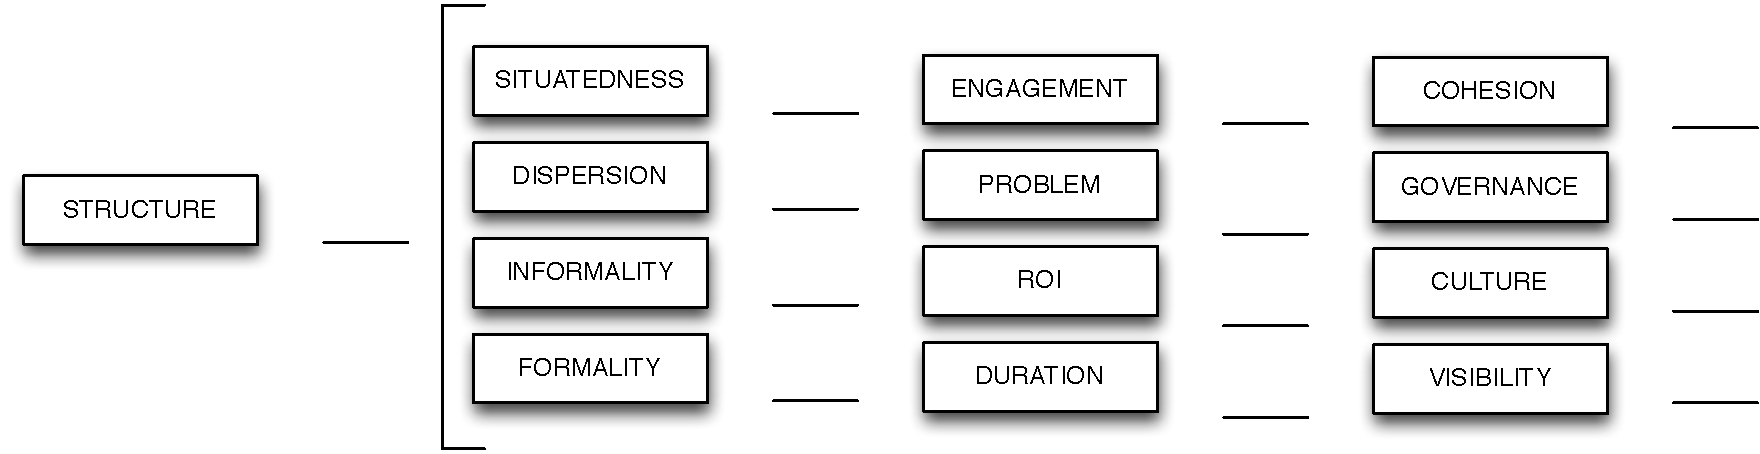
\includegraphics[width=5.3in]{checklist.pdf}    %
%  \end{center}
%\vspace{-.3cm}
\caption{\footnotesize SEEDS: a checklist for essential community information.}\label{checklist}
%\end{wrapfigure}
\end{figure}
\subsection{The SEEDS Decision-Tree}\label{dectree}

Inherited from \cite{specissue} the decision-tree is the essential core of SEEDS. Once data from the questionnaire/checklist is available, the decision-tree can now be used to plot the current configuration of the observed organisation.

%The notion of \emph{key-defining} attribute is not applicable to all cases. What happens if we observe multiple \emph{key-defining} attributes together in a real-life situation? We must then be able to relate this observation to the corresponding social community types. For this reason, SEEDS blends the checklist in Fig.~\ref{checklist} with the decision-tree in Fig.~\ref{tree}, from previous work \cite{specissue}.
%
%Analysing the \emph{key-defining} attributes we found many relations between them: for example, some implied or mutually-excluded others. The relations formed a partial-order function for \emph{key-defining} attributes. A partial-order function associates an ordering or sequencing to the elements of a set. A real-life example of a partially-ordered set is a family genealogical tree, where some pairs of people bear the descendant-ancestor relationship, but not all pairs.
%
%The decision-tree (see Fig.~\ref{tree}) is a representation of the partial-order relationship between \emph{key-defining} attributes. All the relations can be found online\footnote{\url{http://www.fileden.com/files/2012/3/7/3275239/OSSdecision.pdf}}.
%
%The nodes on the tree are labelled with \emph{key-defining} attributes (e.g.~if a ``STRUCTURE'' and ``DISPERSION'' are observable then type NoP is identified). When visiting the tree, the observer needs to decide wether the key defining attributes are present or not. Each decision can be formulated in terms of a question (e.g.~``Do community members use informal communication only?''). These questions can be easily answered by observing any organisation, be it a single development effort, or an entire enterprise. 
%
%The edges of the tree are Yes/No decisions made for each node, from the checklist (see Fig.~\ref{checklist}). 
%The leaves of the tree are social community types (see Table \ref{commtypes}).
%
%\begin{figure}[h!]
%%\begin{wrapfigure}{r}{0.30\textwidth}
%%  \begin{center}
%    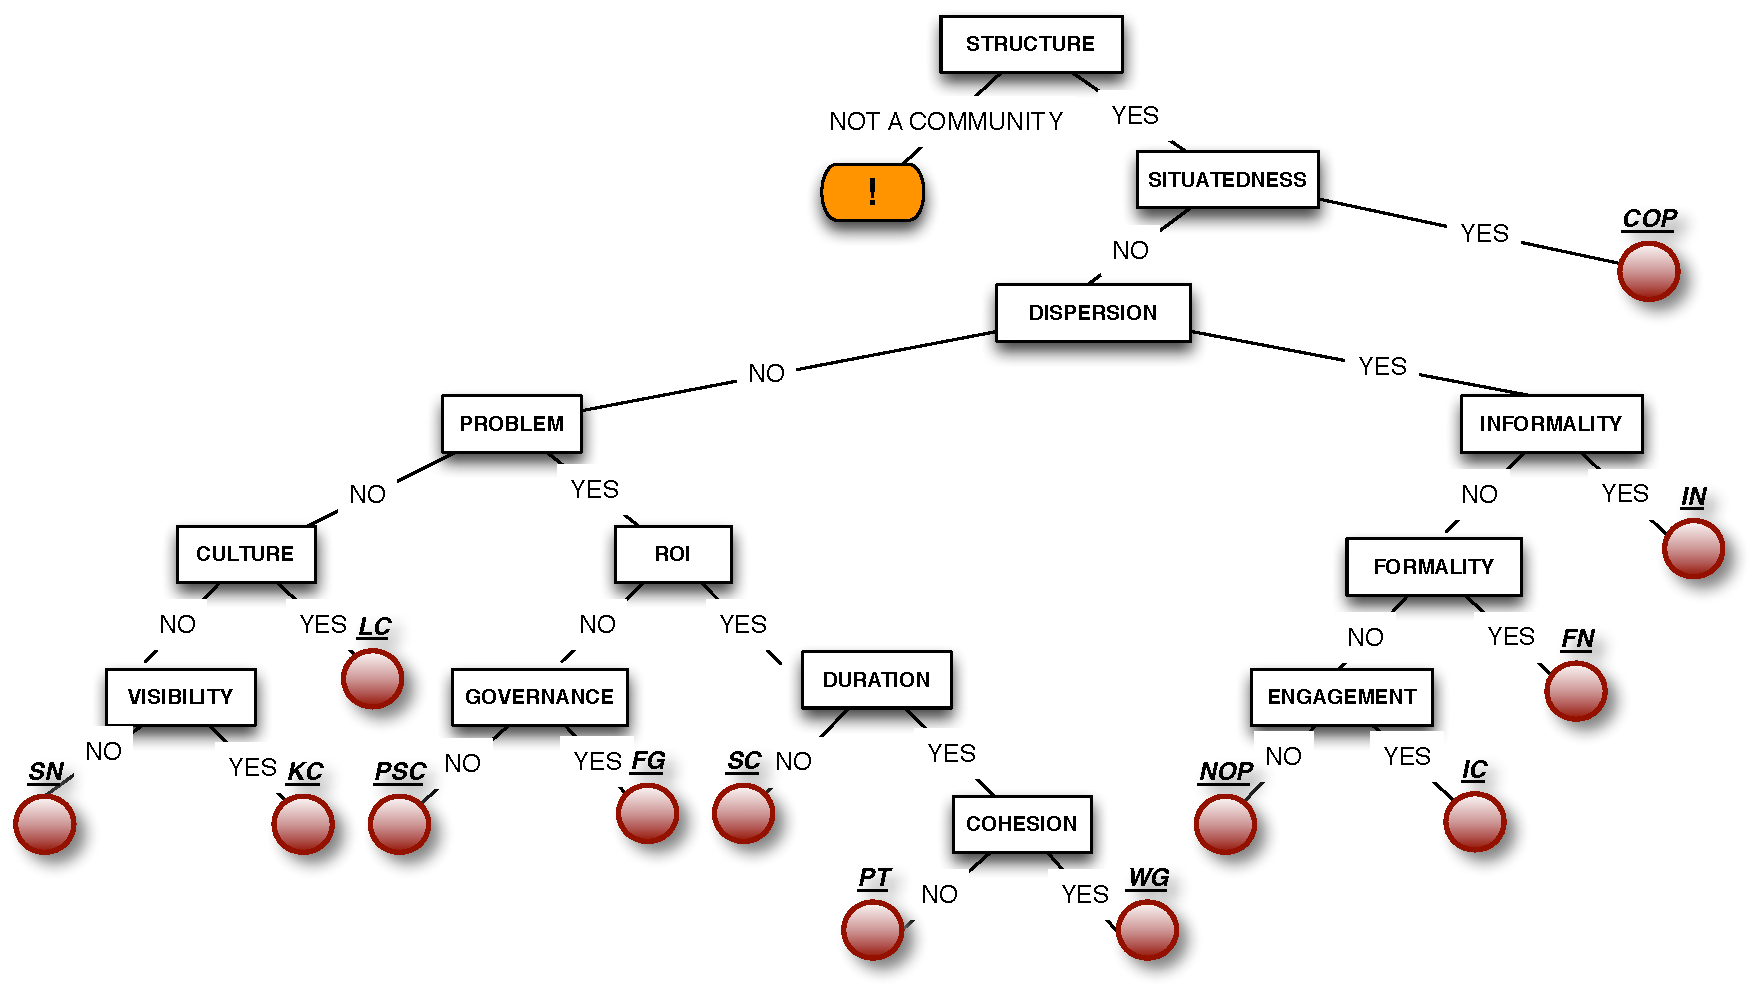
\includegraphics[width=5.3in]{tree.pdf}    %
%%  \end{center}
%%\vspace{-.3cm}
%\caption{\footnotesize SEEDS: a checklist for essential community information.}\label{tree}
%%\end{wrapfigure}
%\end{figure}

\subsection{The SEEDS Analysis Framework}\label{fw}

Inheriting from strategic evaluation approaches such as \cite{swot}, we elaborated an initial analysis framework for SEEDS \emph{snapshots} using evidence and observations from our case-study. To understand strengths, weaknesses, opportunities and threats analysing community properties using SEEDS \emph{snapshots}, there are three key dimensions that must be evaluated.

First, observers must evaluate the \emph{snapshot} form; second, observers must find \emph{desirable properties}; third, finally, observers must verify if the observed community has \emph{higher-order needs}. Figure \ref{fwpic} shows the resulting evaluations that can be performed (on the left-hand side) using either decision-tree forms, desirable properties or higher-order needs (right-hand side).

SEEDS \emph{snapshots} can assume three possible forms:

\begin{enumerate}
\item \emph{Simple}: the answers in the questionnaire reflect a single, clear-cut path on the decision-tree. The community is well delineated and reflected by a type from literature. Additional attributes in the checklist are not present. The scenario exemplified earlier in Section \ref{intro} represents an instance of a simple community \emph{snapshot}. This form evidences a \textbf{strength} and \textbf{opportunity} of the community. The community is well defined and can be ``enriched'' with additional communities (or attributes) in a controlled fashion, e.g.~using additional SEEDS \emph{\emph{snapshots}}. This level of control delivers an advantage compared to other forms. Also, the company can expand the community as needed, using extensions to its advantage.

\item \emph{Enriched-Community}: the answers in the questionnaire reflect one path blended with additional attributes (including pivots) but no additional paths. This form evidences attributes that ``enrich'' the community, and can represent a \textbf{threat} for the community. The additional attributes can be caused by positive emergent circumstances but also harmful ``deviations''. This form can require additional study.
For example, suppose the ``visibility'' attribute is discovered in mix with the Formal Networks community type. Formality within formal networks might have forced the organisation to adopt mechanisms to increase the visibility of projects, people or artefacts, perhaps it is wise to foster the generation of a Knowledge Community jointly with the Formal Network. The enrichments indicate reasons for insufficient communities support. Practitioners can use the evidence to fill-in with missing support. Refinement and explicit support to such technologies includes the adoption of Information Management or Social Networking technologies \cite{eis,eim} to support development community.

\item \emph{Complex}: The answers in the questionnaire reflect more than one path through one (or more) pivot points. The \emph{snapshot} can be used to identify and support explicitly sub-communities. This form evidences possible \textbf{opportunities} for the community. Sub-communities can be identified by analysing deeper available pivots. Information leading to the ``multiple'' answer could be referred only to a specific division or location within the community. For example, suppose you analyse a Global Software Development organisation. Suppose you find a WG and DISPERSION is a pivot-point, that leads to the identification of a NoP. Details leading to a NoP however, when analysed further, are only referred to a single site in the GSD organisation. In case sub-communities are identified, managers can use the \emph{snapshot} to plan explicit support to their attributes.

%
%Pivot-points can also indicate reasons for an inefficient community. Community members show attributes of other communities that were not explicitly planned nor supported.
%\item \emph{complex}: The answers in the questionnaire reflect more than one path and additional attributes.
%\item \emph{chaotic}: The answers in the questionnaire reflect sparse attributes that don't represent any path but only broken segments. This indicates that the community is in some disarray, since it doesn't show any clear organisational form. The community is not representable with known organisational types. The \emph{snapshot} form can be used to identify the attributes that remain unsupported (i.e.~the broken links). For example, suppose you are observing a set of people working almost as a Workgroup but are not required to show any benefit on investments. This shortcoming can be made explicit and further investigated.
\end{enumerate}

% Ref to Ralph Stacey's certainty/agreement matrix. See the summary at http://www.gp-training.net/training/communication_skills/consultation/equipoise/complexity/stacey.htm
This division has many similarities to the Stacey matrix \cite{sta02aa}. We explore this connection in Section~\ref{sec:complexity}.

Second, \emph{\mbox{(un-)desirable} properties} are items in the checklist that were (a) desired but not discovered, or (b) discovered but not desired. For example imagine you expected your community to exhibit increased visibility of its members and resources, but found the VISIBILITY attribute to be NO. This analysis reveals possible \textbf{weaknesses} of the community. Additional properties can be fostered with explicit supportive services (e.g.~using knowledge-bases or enterprise social networks to foster VISIBILITY). Conversely, imagine you found the attribute FORMALITY set to YES but expected there to be more informality in the way of working within your company, e.g.~to foster collaborativeness. Again, this analysis reveals \textbf{weaknesses} of your community. Left uncontrolled, some aspects of the community emerged an undesirable feature. This analysis dimension can be used to fine-tune community governance based on the properties found \emph{\mbox{(un-)desirable} properties}.

Third, finally, the decision-tree can be divided in three areas. 
\begin{enumerate} 
\item \emph{structure:} the first three nodes of the tree, namely STRUCTURE, SITUATEDNESS and DISPERSION, focus on the structure of your community, e.g.~whether it has a situated or dispersed practice.
\item \emph{networking:} the YES-branch out of the DISPERSION node, identifies community archetypes whose purpose is increasing the networking within your organisation or across partner organisations. The community's focus is networking, either autonomously or on-purpose.
\item \emph{goals:} the NO-branch out of the DISPERSION node, identifies community archetypes whose purpose is pursue a particular goal, under certain conditions. The community's focus is its goal (e.g.~an organisational problem or Return-on-Investments).
\end{enumerate}

The three areas or ``foci'' above, are higher-order properties of your community. SEEDS \emph{\emph{snapshots}} can be analysed to identify the missing focus, i.e.~a \emph{Higher-order need}. For example, imagine you take a \emph{snapshot} of your community and find out that the networking ``focus'' is missing but desired. You can use the \emph{snapshot} to identify the missing properties to pursue networking as desired.

\begin{figure}[h!]
%\begin{wrapfigure}{r}{0.30\textwidth}
%  \begin{center}
    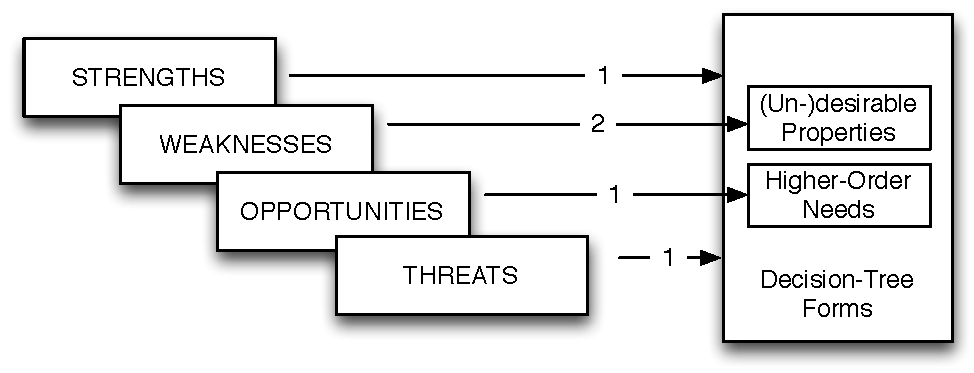
\includegraphics[width=5.4in]{fw.pdf}    %
%  \end{center}
%\vspace{-.3cm}
\caption{\footnotesize SEEDS: an analysis framework.}\label{fwpic}
%\end{wrapfigure}
\end{figure}


% Comment from Martin: this section may only make sense for organisations that have a "desired model".
% MARTIN: add references to literature, written vs lived.
% See f.ex. the competing values framework (Quinn, 1988) or \cite{hoopet93aa}

%
%DRAW A PICTURE OF THE METHOD AND SYNCH THE STRUCTURE OF THE SECTION ON THE PICTURE\\
%FOLLOW THE STRUCTURE OF THE METHOD TO FURTHER INTRODUCE ITS COMPONENTS\\
%EXPLAIN CONSTRUCTION AND RATIONALE OF QUESTIONNAIRE\\
%IN A SEPARATE SUBSECTION EXPLAIN TYPES AND THEIR IDENTIFYING PROPERTIES\\
%EXPLAIN RELATIONS AND CONSTRUCTION OF THE TREE\\